% --------------------------------------------------------------
% This is all preamble stuff that you don't have to worry about.
% Head down to where it says "Start here"
% --------------------------------------------------------------

\documentclass[12pt]{article}

\usepackage[margin=1in]{geometry} 
\usepackage{amsmath,amsthm,amssymb}
\usepackage{comment}
\usepackage{graphicx}

\newcommand{\N}{\mathbb{N}}
\newcommand{\Z}{\mathbb{Z}}

\newenvironment{theorem}[2][Theorem]{\begin{trivlist}
		\item[\hskip \labelsep {\bfseries #1}\hskip \labelsep {\bfseries #2.}]}{\end{trivlist}}
\newenvironment{lemma}[2][Lemma]{\begin{trivlist}
		\item[\hskip \labelsep {\bfseries #1}\hskip \labelsep {\bfseries #2.}]}{\end{trivlist}}
\newenvironment{exercise}[2][Exercise]{\begin{trivlist}
		\item[\hskip \labelsep {\bfseries #1}\hskip \labelsep {\bfseries #2.}]}{\end{trivlist}}
\newenvironment{reflection}[2][Reflection]{\begin{trivlist}
		\item[\hskip \labelsep {\bfseries #1}\hskip \labelsep {\bfseries #2.}]}{\end{trivlist}}
\newenvironment{proposition}[2][Proposition]{\begin{trivlist}
		\item[\hskip \labelsep {\bfseries #1}\hskip \labelsep {\bfseries #2.}]}{\end{trivlist}}
\newenvironment{corollary}[2][Corollary]{\begin{trivlist}
		\item[\hskip \labelsep {\bfseries #1}\hskip \labelsep {\bfseries #2.}]}{\end{trivlist}}

\begin{document}
	
	% --------------------------------------------------------------
	%                         Start here
	% --------------------------------------------------------------
	
	%\renewcommand{\qedsymbol}{\filledbox}
	
	\title{Water Distribution}%replace X with the appropriate number
	\author{Berk Ozturk and Ali Saab
	} %if necessary, replace with your course title
	
	\maketitle
	
	\section{Introduction}
	
	
	\section{Preliminary Optimization Problem}
	
	\subsection{Problem parameters}
	
	
	We define the variables:
	
		\begin{itemize}
		\item N is the number of Nodes
		\item K is the number of available diameter dimensions
		\item $d_{k}$ is the diameter of an available pipe, increasing with $k$

		\item $ConCost$ is the cost of a connection
		\item $\rho$ is density of the fluid
		\item $\mu$ is viscosity of the fluid
		\item g is the gravity
	\end{itemize}
	
	\subsection{Nodal variables}
	
	For $i = [1, ..., N]$, where $N$ is the number of nodes:
	\begin{itemize}
		\item $H_{i}$ is the head at Node $i$
		\item $H_{\rm{min}, i}$ is the minimum head allowed at Node $i$
	\end{itemize}
	
	\section{Edge variables}
	For $i, j = [1, ..., N]$, where $N$ is the number of nodes, 
	we have an edge $i,j$ connecting each pair of nodes. For each edge $i,j$:
	\begin{itemize}
		\item $C_{i,j}$ is the cost between nodes $i$ and $j$
		\item $L_{i,j}$ is the length of the pipe between nodes $i$ and $j$
		\item $\epsilon_{i,j}$ is the roughness of the pipe between nodes $i$ and $j$
		\item $\bar{\epsilon}_{i,j}$ is the relative roughness of the pipe between 	nodes $i$ and $j$
		\item $D_{i,j}$ is the diameter of the pipe between nodes $i$ and $j$
		\item $F_{i,j}$ is the flow rate between from Node $i$ to Node $j$
		\item $M_{i,j}$ is the maximum flow rate between from Node $i$ to Node $j$
		\item $V_{i,j}$ is the velocity of the flow from Node $i$ to Node $j$
		\item $h_{i,j}$ is the head loss due to the flow from Node $i$ to Node $j$
		\item $Re_{i,j}$ is the Reynold's Number of the flow from Node $i$ to Node $j$
		\item $f_{i,j}$ is the Darcy friction factor of the flow from Node $i$ to Node $j$
		\item $Con_{i,j}$ indicates whether a connection exists from Node $i$ to Node $j$
	\end{itemize}
	
	\begin{equation}
	\begin{aligned}
	& \min &&\sum_{i=1}^{N}\sum_{j=1}^{N} F_{i,j} C_{i,j} &&+ Con_{i,j} ConCost\\
	& \text{ s.t.} && \sum_{j \neq i} F_{i,j} && = \sum_{j \neq i} F_{j,i} \quad && i = 1, 2, ... N\\
	& && \sum_{j \neq i} H_j Con_{j,i} && = H_i + \sum_{J \neq i} h_{j,i}Con_{j,i} && i = 1,2, ...N\\
	& && H_i && \geq H_{\rm{min}} && i = 1, 2, ..., N \\
	& && C_{i,j} && = 1.1 D_{i,j}^{1.5} L_{i,j} && i = 1, 2, ..., N \quad && j = 1, 2, ... N\\
	& && F_{i,j} && \leq M_{i,j} Con_{i,j} && i = 1, 2, ..., N \quad && j = 1, 2, ... N\\
	& && F_{i,j} && \geq 0 && i = 1, 2, ..., N \quad && j = 1, 2, ... N\\
	& && Con_{i,j}Con_{j,i} && \leq 10^{-30} && i = 1, 2, ..., N \quad && j = i+1, ... N\\
	& && Con_{i,j} &&\in \{0,1\} && i = 1, 2, ..., N \quad && j = 1, 2, ... N\\
	& && h_{i,j} && = \frac{f_{i,j} L_{i,j} V_{i,j}^2}{2D_{i,j} g} && i = 1, 2, ..., N \quad && j = 1, 2, ... N\\
	& && V_{i,j} && = \frac{4 F_{i,j}}{\pi D_{i,j}^2} && i = 1, 2, ..., N \quad && j = 1, 2, ... N\\
	& && f_{i,j} &&= \frac{0.25}{\log\left(\frac{\bar{\epsilon}}{3.7} + \frac{5.74}{Re_{i,j}^{0.9}}\right)^2} && i = 1, 2, ..., N \quad && j = 1, 2, ... N\\
	& && \bar{\epsilon}_{i,j} && = \frac{\epsilon_{i,j}}{D_{i,j}} && i = 1, 2, ..., N \quad && j = 1, 2, ... N\\
	& && Re_{i,j} && = \frac{\rho V_{i,j} D_{i,j}}{\mu} && i = 1, 2, ..., N \quad && j = 1, 2, ... N\\
	& && D_{i,j} && = D_{j,i} && i = 1, 2, ..., N \quad && j = i+1, ... N\\
	& && D_{i,j} && = \sum_{k=1}^{K}x_{i,j,k}d_k && i = 1, 2, ..., N \quad && j = 1, 2, ... N\\
	& && \sum_{k=1}^{K} x_{i,j,k} && \leq 1 && i = 1, 2, ..., N \quad && j = 1, 2, ... N\\
	& && x_{i,j,k} && \in \{0,1\} && i = 1, 2, ..., N \quad && j = 1, 2, ... N \\
	& && && && k = 1,2, ..K\\ 
	\end{aligned}
	\end{equation}
	

	
	The above optimization problem should be modified to become more tractable.
	
	\section{Modifying Constraints}
	\begin{comment}
	\subsection{Integrality of Connection variable}
	The constraints
	\begin{equation}
	\begin{aligned}
	& Con_{i,j} + Con_{j,i} && \leq 1 && i = 1, 2, ..., N \quad && j = i+1, ... N\\
	& Con_{i,j} &&\in \{0,1\} && i = 1, 2, ..., N \quad && j = 1, 2, ... N\\
	\end{aligned}
	\end{equation}
	
	can be replaced by
	
	\begin{equation}
	\begin{aligned}
	& Con_{i,j} && \leq 1 && i = 1, 2, ..., N \quad && j = 1, 2, ... N\\
	& Con_{i,j} && \geq 0 && i = 1, 2, ..., N \quad && j = 1, 2, ... N\\
	& Con_{i,j}*Con_{j,i} && \leq 0 && i = 1, 2, ..., N \quad && j = i+1, ... N\\
	\end{aligned}
	\end{equation}
	and the requirement on minimal head at each Node will drive the connections between some nodes to be non-zero. Note that for predefined topologies, those constraints are not needed since the connections will be given as an input.
	\end{comment}
	\subsection{Relaxing the Diameter Constraint}
	The constraint 
	\begin{equation}
	D_{i,j} = \sum_{k=1}^{K}x_{i,j,k}d_k \quad i = 1, 2, ..., N \quad j = 1, 2, ... N
	\end{equation}
	
	Can be relaxed and replaced by 
	\begin{equation}
	D_{i,j} \geq \sum_{k=1}^{K}x_{i,j,k}d_k \quad i = 1, 2, ..., N \quad j = 1, 2, ... N
	\end{equation}
	
	Since the diameter tends to be smaller as the cost and flow rate increases with the increase in diameter.
	
	\subsection{Non GP compatible constraints}
	The three non GP compatible constraints are 
	\begin{equation}
	\begin{aligned}
	& \sum_{j \neq i} F_{i,j} && = \sum_{j \neq i} F_{j,i} \quad && i = 1, 2, ... N\\
	& \sum_{j \neq i} H_j Con_{j,i} && = H_i + \sum_{J \neq i} h_{j,i}Con_{j,i} && i = 1,2, ...N\\
	& f_{i,j} &&= \frac{0.25}{\log\left(\frac{\bar{\epsilon}_{i,j}}{3.7} + \frac{5.74}{Re_{i,j}^{0.9}}\right)^2} && i = 1, 2, ..., N \quad && j = 1, 2, ... N\\
	\end{aligned}
	\end{equation}
	The second signomial equality constraint can be relaxed as follows
	\begin{equation}
	\sum_{j \neq i} H_j Con_{j,i} \geq H_i + \sum_{J \neq i} h_{j,i}Con_{j,i} \quad i = 1,2, ...N\\
	\end{equation}
	Since the Head at each Node tends to be larger. This is still a non GP compatible in general, however a signomial inequality is better than a signomial equality.
	
	using slack variables, the first constraint will be replaced by the following
	\begin{equation}
	\begin{aligned}
	& \sum_{j \neq i} F_{i,j} && \leq S_{1,i}(\sum_{j \neq i} F_{j,i}) \quad && i = 1, 2, ... N\\
	& S_{\rm{out},i}(\sum_{j \neq i} F_{i,j}) && \geq \sum_{j \neq i} F_{j,i} \quad && i = 1, 2, ... N\\
	& S_{1,i} && \geq 1 \quad && i = 1, 2, ... N\\
	& S_{\rm{out},i} && \geq 1 \quad && i = 1, 2, ... N\\
	\end{aligned}
	\end{equation}
	and the objective function will be modified as follows
	\begin{equation}
	(\sum_{i=1}^{N}\sum_{j=1}^{N} F_{i,j} C_{i,j} + Con_{i,j} ConCost)(1 + slackCost \prod_{i=1}^{N}S_{1,i}S_{\rm{out},i})
	\end{equation}
	Where the parameter $slackCost$ might need tuning for some problems.
	
	The last constraint can also be relaxed as follows
	\begin{equation}
	f_{i,j} \geq \frac{0.25}{\log\left(\frac{\bar{\epsilon}_{i,j}}{3.7} + \frac{5.74}{Re_{i,j}^{0.9}}\right)^2} \quad i = 1, 2, ..., N \quad j = 1, 2, ... N\\
	\label{fricRel}
	\end{equation}
	As the friction factor will try to be as low as possible to decrease friction.
	
	The right hand of equation \eqref{fricRel} is convex in log-space for the region of interest as shown below
	\begin{figure}
		\centering
		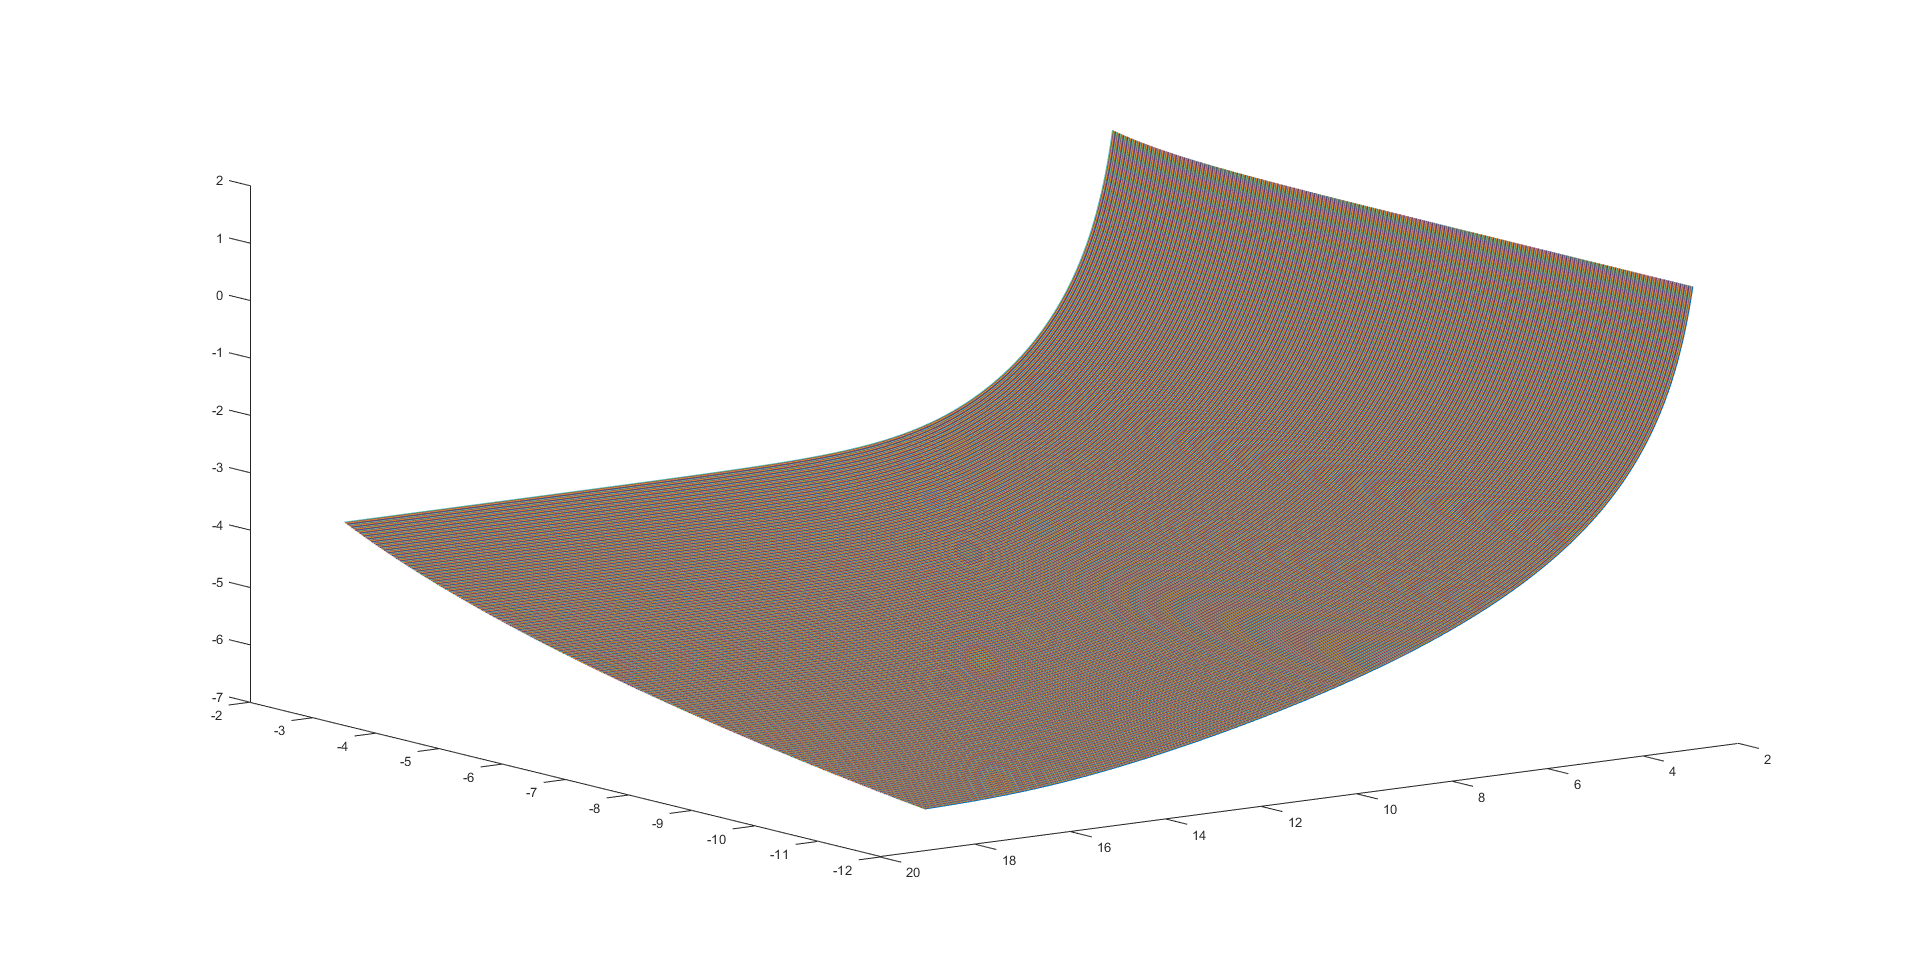
\includegraphics[scale=0.3]{frictionFactorLogSpace.png}
		\caption{Friction Factor RHS is convex}
		\label{fig:fricFactorLogSpace}
	\end{figure}
	The above constraint can fitted to a posynomial constraint using softmax affine functions, and the resulting constraint is as follows
	
	\begin{equation}
	f \geq posy
	\end{equation}
	
	with an RMS error of something between $Re = 10^3$ and $10^8$, and relative roughness between $10^-5$ and $0.1$
	
	\newpage
	
	\section{Final Optimization Problem}
	
	The resulting Mixed Integer Signomial Optimization Problem is as follows
	
	\begin{equation}
	\begin{aligned}
	&\min &&(\sum_{i=1}^{N}\sum_{j=1}^{N} F_{i,j} C_{i,j} && + Con_{i,j} ConCost)(1 + slackCost &&\prod_{i=1}^{N}S_{1,i}S_{\rm{out},i})\\
	& \text{ s.t.} && \sum_{j \neq i} F_{i,j} && \leq S_{\rm{in},i}(\sum_{j \neq i} F_{j,i}) \quad && i = 1, 2, ... N\\
	& && S_{\rm{out},i}(\sum_{j \neq i} F_{i,j}) && \geq \sum_{j \neq i} F_{j,i} \quad && i = 1, 2, ... N\\
	& && S_{\rm{in},i} && \geq 1 \quad && i = 1, 2, ... N\\
	& && S_{\rm{out},i} && \geq 1 \quad && i = 1, 2, ... N\\
	& && \sum_{j \neq i} H_j Con_{j,i} && \geq H_i + \sum_{J \neq i} h_{j,i}Con_{j,i} && i = 1,2, ...N\\
	& && H_i && \geq H_{\rm{min}} && i = 1, 2, ..., N \\
	& && C_{i,j} && = 1.1 D_{i,j}^{1.5} L_{i,j} && i = 1, 2, ..., N \quad && j = 1, 2, ... N\\
	& && F_{i,j} && \leq M_{i,j} Con_{i,j} && i = 1, 2, ..., N \quad && j = 1, 2, ... N\\
	& && F_{i,j} && \geq 0 && i = 1, 2, ..., N \quad && j = 1, 2, ... N\\
	& && Con_{i,j}Con_{j,i} && \leq 10^{-30} && i = 1, 2, ..., N \quad && j = i+1, ... N\\
	& && Con_{i,j} &&\in \{0,1\} && i = 1, 2, ..., N \quad && j = 1, 2, ... N\\
	& && h_{i,j} && = \frac{f_{i,j} L_{i,j} V_{i,j}^2}{2D_{i,j} g} && i = 1, 2, ..., N \quad && j = 1, 2, ... N\\
	& && V_{i,j} && = \frac{4 F_{i,j}}{\pi D_{i,j}^2} && i = 1, 2, ..., N \quad && j = 1, 2, ... N\\
	& && f_{i,j} &&\geq posy(\bar{\epsilon}_{i,j}, Re_{i,j}) && i = 1, 2, ..., N \quad && j = 1, 2, ... N\\
	& && \bar{\epsilon}_{i,j} && = \frac{\epsilon_{i,j}}{D_{i,j}} && i = 1, 2, ..., N \quad && j = 1, 2, ... N\\
	& && Re_{i,j} && = \frac{\rho V_{i,j} D_{i,j}}{\mu} && i = 1, 2, ..., N \quad && j = 1, 2, ... N\\
	& && D_{i,j} && = D_{j,i} && i = 1, 2, ..., N \quad && j = i+1, ... N\\
	& && D_{i,j} && \geq \sum_{k=1}^{K}x_{i,j,k}d_k && i = 1, 2, ..., N \quad && j = 1, 2, ... N\\
	& && \sum_{k=1}^{K} x_{i,j,k} && \leq 1 && i = 1, 2, ..., N \quad && j = 1, 2, ... N\\
	& && x_{i,j,k} && \in \{0,1\} && i = 1, 2, ..., N \quad && j = 1, 2, ... N \\
	& && && && k = 1,2, ..K\\ 
	\end{aligned}
	\end{equation}
	
	\section{Hanoi Water Distribution Network}
	
	For the Hanoi Water Distribution Network, the topology is known, then the variable Con is predefined, and therefore the two constraints
	\begin{equation}
	\begin{aligned}
	& && Con_{i,j}Con_{j,i} && \leq 10^{-30} && i = 1, 2, ..., N \quad && j = i+1, ... N\\
	& && Con_{i,j} &&\in \{0,1\} && i = 1, 2, ..., N \quad && j = 1, 2, ... N\\
	\end{aligned}
	\end{equation}
	Can be removed. Therefore, the only integer variables involved now are those corresponding to the diameter dimensions $x_{i,j,k}$.
	
	The Hanoi Water Distribution Network can be modeled as follows:
	
	\begin{equation}
	\begin{aligned}
	&\min &&(\sum_{i=1}^{N}\sum_{j=1}^{N} F_{i,j} C_{i,j})&&(1 + slackCost \prod_{i=1}^{N}S_{\rm{in},i}S_{\rm{out},i})\\
	& \text{ s.t.} && \sum_{j \neq i} F_{i,j} && \leq S_{\rm{in},i}(\sum_{j \neq i} F_{j,i}) \quad && i = 1, 2, ... N\\
	& && S_{\rm{out},i}(\sum_{j \neq i} F_{i,j}) && \geq \sum_{j \neq i} F_{j,i} \quad && i = 1, 2, ... N\\
	& && S_{\rm{in},i} && \geq 1 \quad && i = 1, 2, ... N\\
	& && S_{\rm{out},i} && \geq 1 \quad && i = 1, 2, ... N\\
	& && \sum_{j \neq i} H_j Con_{j,i} && \geq H_i + \sum_{J \neq i} h_{j,i}Con_{j,i} && i = 1,2, ...N\\
	& && H_i && \geq H_{\rm{min}} && i = 1, 2, ..., N \\
	& && C_{i,j} && = 1.1 D_{i,j}^{1.5} L_{i,j} && i = 1, 2, ..., N \quad && j = 1, 2, ... N\\
	& && F_{i,j} && \leq M_{i,j} Con_{i,j} && i = 1, 2, ..., N \quad && j = 1, 2, ... N\\
	& && F_{i,j} && \geq 0 && i = 1, 2, ..., N \quad && j = 1, 2, ... N\\
	& && h_{i,j} && = \frac{f_{i,j} L_{i,j} V_{i,j}^2}{2D_{i,j} g} && i = 1, 2, ..., N \quad && j = 1, 2, ... N\\
	& && V_{i,j} && = \frac{4 F_{i,j}}{\pi D_{i,j}^2} && i = 1, 2, ..., N \quad && j = 1, 2, ... N\\
	& && f_{i,j} &&\geq posy(\bar{\epsilon}_{i,j}, Re_{i,j}) && i = 1, 2, ..., N \quad && j = 1, 2, ... N\\
	& && \bar{\epsilon}_{i,j} && = \frac{\epsilon_{i,j}}{D_{i,j}} && i = 1, 2, ..., N \quad && j = 1, 2, ... N\\
	& && Re_{i,j} && = \frac{\rho V_{i,j} D_{i,j}}{\mu} && i = 1, 2, ..., N \quad && j = 1, 2, ... N\\
	& && D_{i,j} && = D_{j,i} && i = 1, 2, ..., N \quad && j = i+1, ... N\\
	& && D_{i,j} && \geq \sum_{k=1}^{K}x_{i,j,k}d_k && i = 1, 2, ..., N \quad && j = 1, 2, ... N\\
	& && \sum_{k=1}^{K} x_{i,j,k} && \leq 1 && i = 1, 2, ..., N \quad && j = 1, 2, ... N\\
	& && x_{i,j,k} && \in \{0,1\} && i = 1, 2, ..., N \quad && j = 1, 2, ... N \\
	& && && && k = 1,2, ..K\\ 
	\end{aligned}
	\end{equation}
	
	Where $\epsilon_{i,j}$, $L_{i,j}$, $\rho$, $\mu$, and $g$ are given, N = 32, and K = 6 with $\{d_k\}_{k=1}^{K}$ given. 
	
	% --------------------------------------------------------------
	%     You don't have to mess with anything below this line.
	% --------------------------------------------------------------
	
\end{document}